\documentclass[a4paper, 12pt]{article}%тип документа

%отступы
\usepackage[left=1cm,right=1cm,top=1cm,bottom=2cm,bindingoffset=0cm]{geometry}

%Русский язык
\usepackage[T2A]{fontenc} %кодировка
\usepackage[utf8]{inputenc} %кодировка исходного кода
\usepackage[english,russian]{babel} %локализация и переносы

%Вставка картинок
\usepackage{graphicx}
\graphicspath{{pictures/}}
\DeclareGraphicsExtensions{.pdf,.png,.jpg}

%Графики
\usepackage{pgfplots}
\pgfplotsset{compat=1.9}

%Математика
\usepackage{amsmath, amsfonts, amssymb, amsthm, mathtools}

%Заголовок
\author{Валеев Рауф Раушанович \\
группа 825}
\title{\textbf{Работа 1.2.5 \\
Исследование вынужденной регулярной прецессии гироскопа}}

\begin{document}
\maketitle
\newpage
\textbf{Цель работы:} исследовать вынужденную прецессию гироскопа; установить зависимость скорости вынужденной прецессии от велечины момента сил, действующих на ось гироскопа; определить скорость вращения ротора гироскопа и сравнить ее со скоростью, расчитанной по скорости прецессии.

\textbf{В работе используются:} гироскоп в кардановом подвесе, секундомер, набор грузов, отдельный ротор гироскопа, цилиндр известной массы, крутильный маятник, штангенциркуль, линейка. 

\textbf{Примерный вид установки}\\
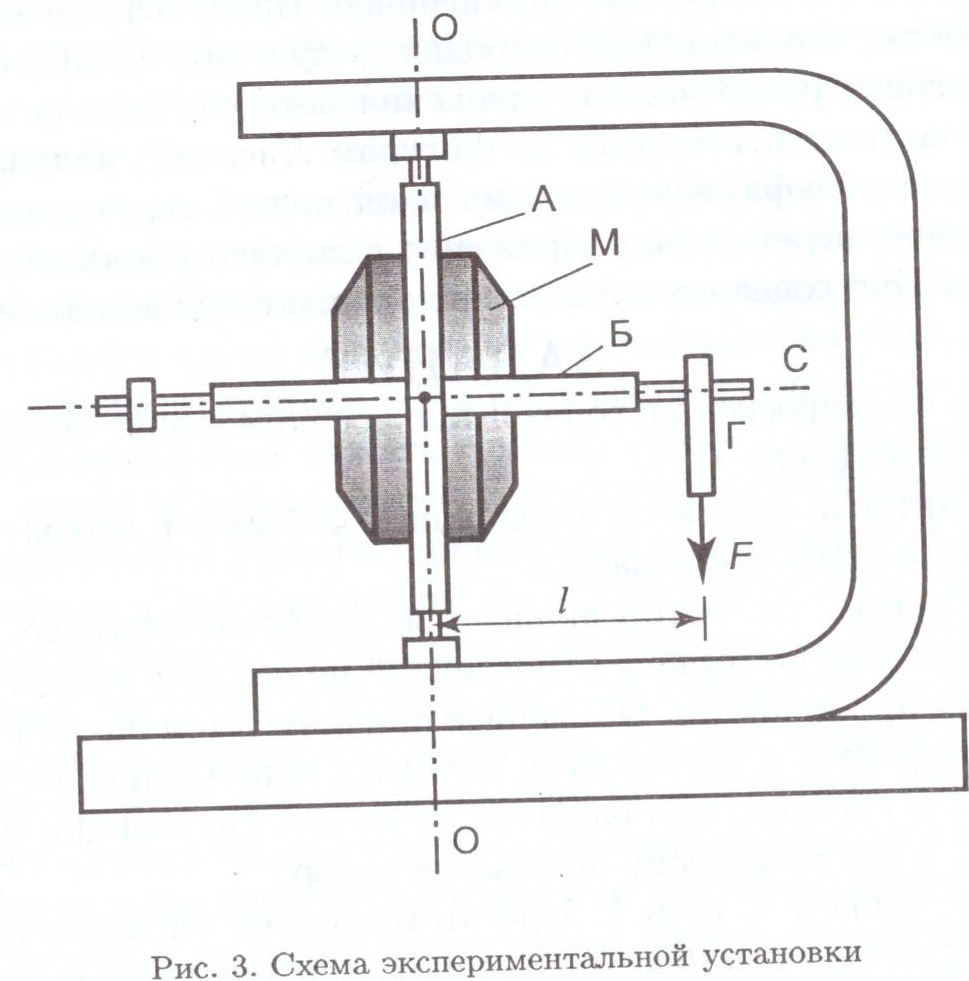
\includegraphics[width=0.4\textwidth]{125_1.jpg}
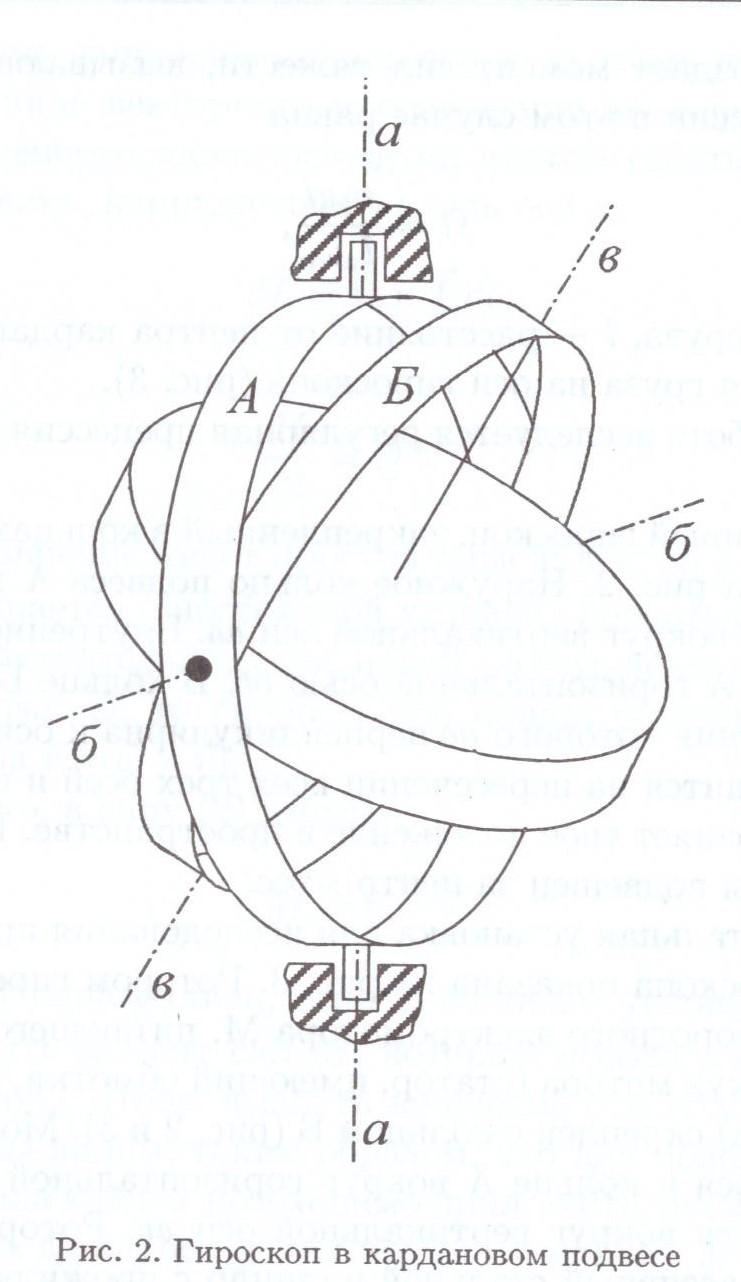
\includegraphics[width=0.4\textwidth]{125_2.jpg}
\begin{enumerate}
\item Устанавливаем ось гироскопа в горизонтальное положение, поворачивая его за рычаг C. 
\item Включаем питание гироскопа и ждем, пока вращение ротора не стабилизируется. 
\item Убеждаемся в том, что ротор вращается достаточно быстро: при легком постукивании по рычагу С последний не должен изменять своего положения в пространстве. \\
Причина: Он не двигается вниз из-за прецессии гироскопа, так как если мы давим вниз или вверх, то момент инерции оси гироскопа направлен по касательной. Он не двигается вбок из-за силы трения в оси ОО. \\
Как движется гироскоп при нажатии на рычаг?
При нажатии сверху гироскоп вращается вниз, при нажатии снизу – ввверх. Отсюда сигма по оси направлена в сторону центра, отсюда гироскоп вращается по часовой стрелке.
\item Подвешиваем к рычагу С груз Г. При этом должна начяться прецессия гироскопа. Трение в оси (в ОО) приводит к тому, что рычаг С начинает медленно опускаться. 
\item Отклоняем гироскоп на 5-6 градусов и измеряем угловую скорость регулярной прецессии $\Omega$. Продолжаем измерения, пока рычаг не отклонится на 5-6 градусов ниже горизонтальной плоскости. Также измеряем скорость рычага С.
\begin{center}
\begin{tabular}{|c|c|c|c|c|c|c|c|}
\hline
\multicolumn{1}{|c|}{$m, g$} & \multicolumn{3}{c|}{180}                          & $M, H \cdot m$   & \multicolumn{3}{c|}{0,21}                                                                        \\ \hline
                             & $N$ & $t, c$                      & $\sigma_t, c$ & $\omega, c^{-1}$ & $\sigma_{\omega}, 10^{-5} \cdot c^{-1}$ & $v, 10^{-5} \cdot m/c$ & $\sigma_v, 10^{-8} \cdot m/c$ \\ \hline
1                            & 4   & 267,5                       &0,1&0,09391          & 3,5                                     & 9,469                  & 8,6                           \\ \hline
2                            & 4   & 267,4                       & 0,1           & 0,09394          & 3,5                                     & 9,472                  & 8,6                           \\ \hline
3                            & 4   & 267,3                       & 0,1           & 0,09397          & 3,5                                     & 9,476                  & 8,6                           \\ \hline
4                            & 4   & 267,5                       & 0,1           & 0,09391          & 3,5                                     & 9,469                  & 8,6                           \\ \hline
5                            & 4   & 267                         & 0,1           & 0,09408          & 3,5                                     & 9,487                  & 8,6                           \\ \hline
Среднее                      & 4   & \multicolumn{1}{l|}{267,3} & 0,1           & 0,09396          & 3,5                                     & 9,475                  & 8,6                           \\ \hline
\end{tabular}
\end{center}
\item Проделываем пункт 5 для 5-7 различных значениях моментов сил.
\begin{center}
\begin{tabular}{|c|c|c|c|c|c|c|c|}
\hline
\multicolumn{1}{|c|}{$m, g$} & \multicolumn{3}{c|}{216}                          & $M, H \cdot m$   & \multicolumn{3}{c|}{0,23}                                                                        \\ \hline
                             & $N$ & $t, c$                      & $\sigma_t, c$ & $\omega, c^{-1}$ & $\sigma_{\omega}, 10^{-5} \cdot c^{-1}$ & $v, 10^{-4} \cdot m/c$ & $\sigma_v, 10^{-7} \cdot m/c$ \\ \hline
1                            & 3   & 201,3                       & 0,1           & 0,09359      & 4,6                                     & 1,258                  & 1,2                           \\ \hline
2                            & 3   & 200,2                       & 0,1           & 0,09411     & 4,7                                     & 1,265                  & 1,2                           \\ \hline
3                            & 3   & 201,2                       & 0,1           & 0,09364    & 4,6                                     & 1,259                  & 1,2                           \\ \hline
4                            & 3   & 200,5                       & 0,1           & 0,09397     & 4,7                                     & 1,263                  & 1,2                           \\ \hline
5                            & 3   & 200,7                       & 0,1           & 0,09387       & 4,7                                     & 1,262                  & 1,2                           \\ \hline
Среднее                      & 3   & \multicolumn{1}{l|}{200,8} & 0,1           & 0,09383      & 4,7                                     & 1,262                  & 1,2                           \\ \hline
\hline
$m, g$  & \multicolumn{3}{c|}{614}     & $M, H \cdot m$   & \multicolumn{3}{c|}{0,66}                                                                        \\ \hline
        & $N$ & $t, c$ & $\sigma_t, c$ & $\omega, c^{-1}$ & $\sigma_{\omega}, 10^{-4} \cdot c^{-1}$ & $v, 10^{-4} \cdot m/c$ & $\sigma_v, 10^{-7} \cdot m/c$ \\ \hline
1       & 6   & 133    & 0,1           & 0,2833           & 2,1                                     & 1,904                  & 2                             \\ \hline
2       & 6   & 133,5  & 0,1           & 0,2822           & 2,1                                     & 1,897                  & 2                             \\ \hline
3       & 6   & 133,7  & 0,1           & 0,2818           & 2,1                                     & 1,894                  & 2                             \\ \hline
4       & 6   & 133,5  & 0,1           & 0,2822           & 2,1                                     & 1,897                  & 2                             \\ \hline
5       & 6   & 133,6  & 0,1           & 0,2821           & 2,1                                     & 1,896                  & 2                             \\ \hline
Среднее & 6   & 133,5 & 0,1           & 0,2823           & 2,1                                     & 1,898                  & 2                             \\ \hline
\hline
$m, g$  & \multicolumn{3}{c|}{142}     & $M, H \cdot m$   & \multicolumn{3}{c|}{0,17}                                                                        \\ \hline
        & $N$ & $t, c$ & $\sigma_t, c$ & $\omega, c^{-1}$ & $\sigma_{\omega}, 10^{-5} \cdot c^{-1}$ & $v, 10^{-5} \cdot m/c$ & $\sigma_v, 10^{-8} \cdot m/c$ \\ \hline
1       & 3   & 253,4  & 0,1           & 0,074349         & 3                                       & 9,996                  & 9                             \\ \hline
2       & 3   & 253,4  & 0,1           & 0,074349         & 3                                       & 9,996                  & 9                             \\ \hline
3       & 3   & 253,3  & 0,1           & 0,074378         & 3                                       & 9,999                  & 9                             \\ \hline
4       & 3   & 253,5  & 0,1           & 0,074320         & 3                                       & 9,992                  & 9                             \\ \hline
5       & 3   & 253,4  & 0,1           & 0,074349         & 3                                       & 9,995                  & 9                             \\ \hline
Среднее & 3   & 253,4  & 0,1           & 0,074349         & 3                                       & 9,996                  & 9                             \\ \hline
\hline
$m, g$  & \multicolumn{3}{c|}{273}     & $M, H \cdot m$   & \multicolumn{3}{c|}{0,32}                                                                        \\ \hline
        & $N$ & $t, c$ & $\sigma_t, c$ & $\omega, c^{-1}$ & $\sigma_{\omega}, 10^{-5} \cdot c^{-1}$ & $v, 10^{-4} \cdot m/c$ & $\sigma_v, 10^{-7} \cdot m/c$ \\ \hline
1       & 4   & 175,2  & 0,1           & 0,14338          & 8                                       & 1,446                  & 1,5                           \\ \hline
2       & 4   & 175    & 0,1           & 0,14354          & 8                                       & 1,447                  & 1,5                           \\ \hline
3       & 4   & 175,6  & 0,1           & 0,14305          & 8                                       & 1,442                  & 1,5                           \\ \hline
4       & 4   & 176    & 0,1           & 0,14273          & 8                                       & 1,440                  & 1,5                           \\ \hline
5       & 4   & 175,5  & 0,1           & 0,14313          & 8                                       & 1,444                  & 1,5                           \\ \hline
Среднее & 4   & 175,5 & 0,1           & 0,14316          & 8                                       & 1,444                  & 1,5                           \\ \hline

\hline
$m, g$  & \multicolumn{3}{c|}{341}     & $M, H \cdot m$   & \multicolumn{3}{c|}{0,37}                                                                        \\ \hline
        & $N$ & $t, c$ & $\sigma_t, c$ & $\omega, c^{-1}$ & $\sigma_{\omega}, 10^{-5} \cdot c^{-1}$ & $v, 10^{-4} \cdot m/c$ & $\sigma_v, 10^{-7} \cdot m/c$ \\ \hline
1       & 5   & 178,3  & 0,1           & 0,17611          & 10                                      & 1,421                  & 1,5                           \\ \hline
2       & 5   & 179    & 0,1           & 0,17542          & 10                                      & 1,415                  & 1,5                           \\ \hline
3       & 5   & 178,5  & 0,1           & 0,17591          & 10                                      & 1,419                  & 1,5                           \\ \hline
4       & 5   & 178,7  & 0,1           & 0,17571          & 10                                      & 1,417                  & 1,5                           \\ \hline
5       & 5   & 178,4  & 0,1           & 0,17601          & 10                                      & 1,419                  & 1,5                           \\ \hline
Среднее & 5   & 178,6  & 0,1           & 0,17583          & 10                                      & 1,418                  & 1,5                           \\ \hline
\end{tabular}

\begin{tabular}{|c|c|c|c|}
\hline
$M, H \cdot m$ & $\sigma_M, H \cdot m$ & $\omega, c^{-1}$ & $\sigma_{\omega}, 10^{-5} \cdot c^{-1}$ \\ \hline
0,21       & 0,01                  & 0,09396          & 3,5                                     \\ \hline
0,23       & 0,01                  & 0,09383          & 5                                     \\ \hline
0,66       & 0,03                  & 0,28233          & 21                                      \\ \hline
0,17      & 0,01                  & 0,07435          & 3                                       \\ \hline
0,32      & 0,015                 & 0,14317          & 8                                       \\ \hline
0,37      & 0,02                  & 0,17583          & 10                                      \\ \hline
\end{tabular}
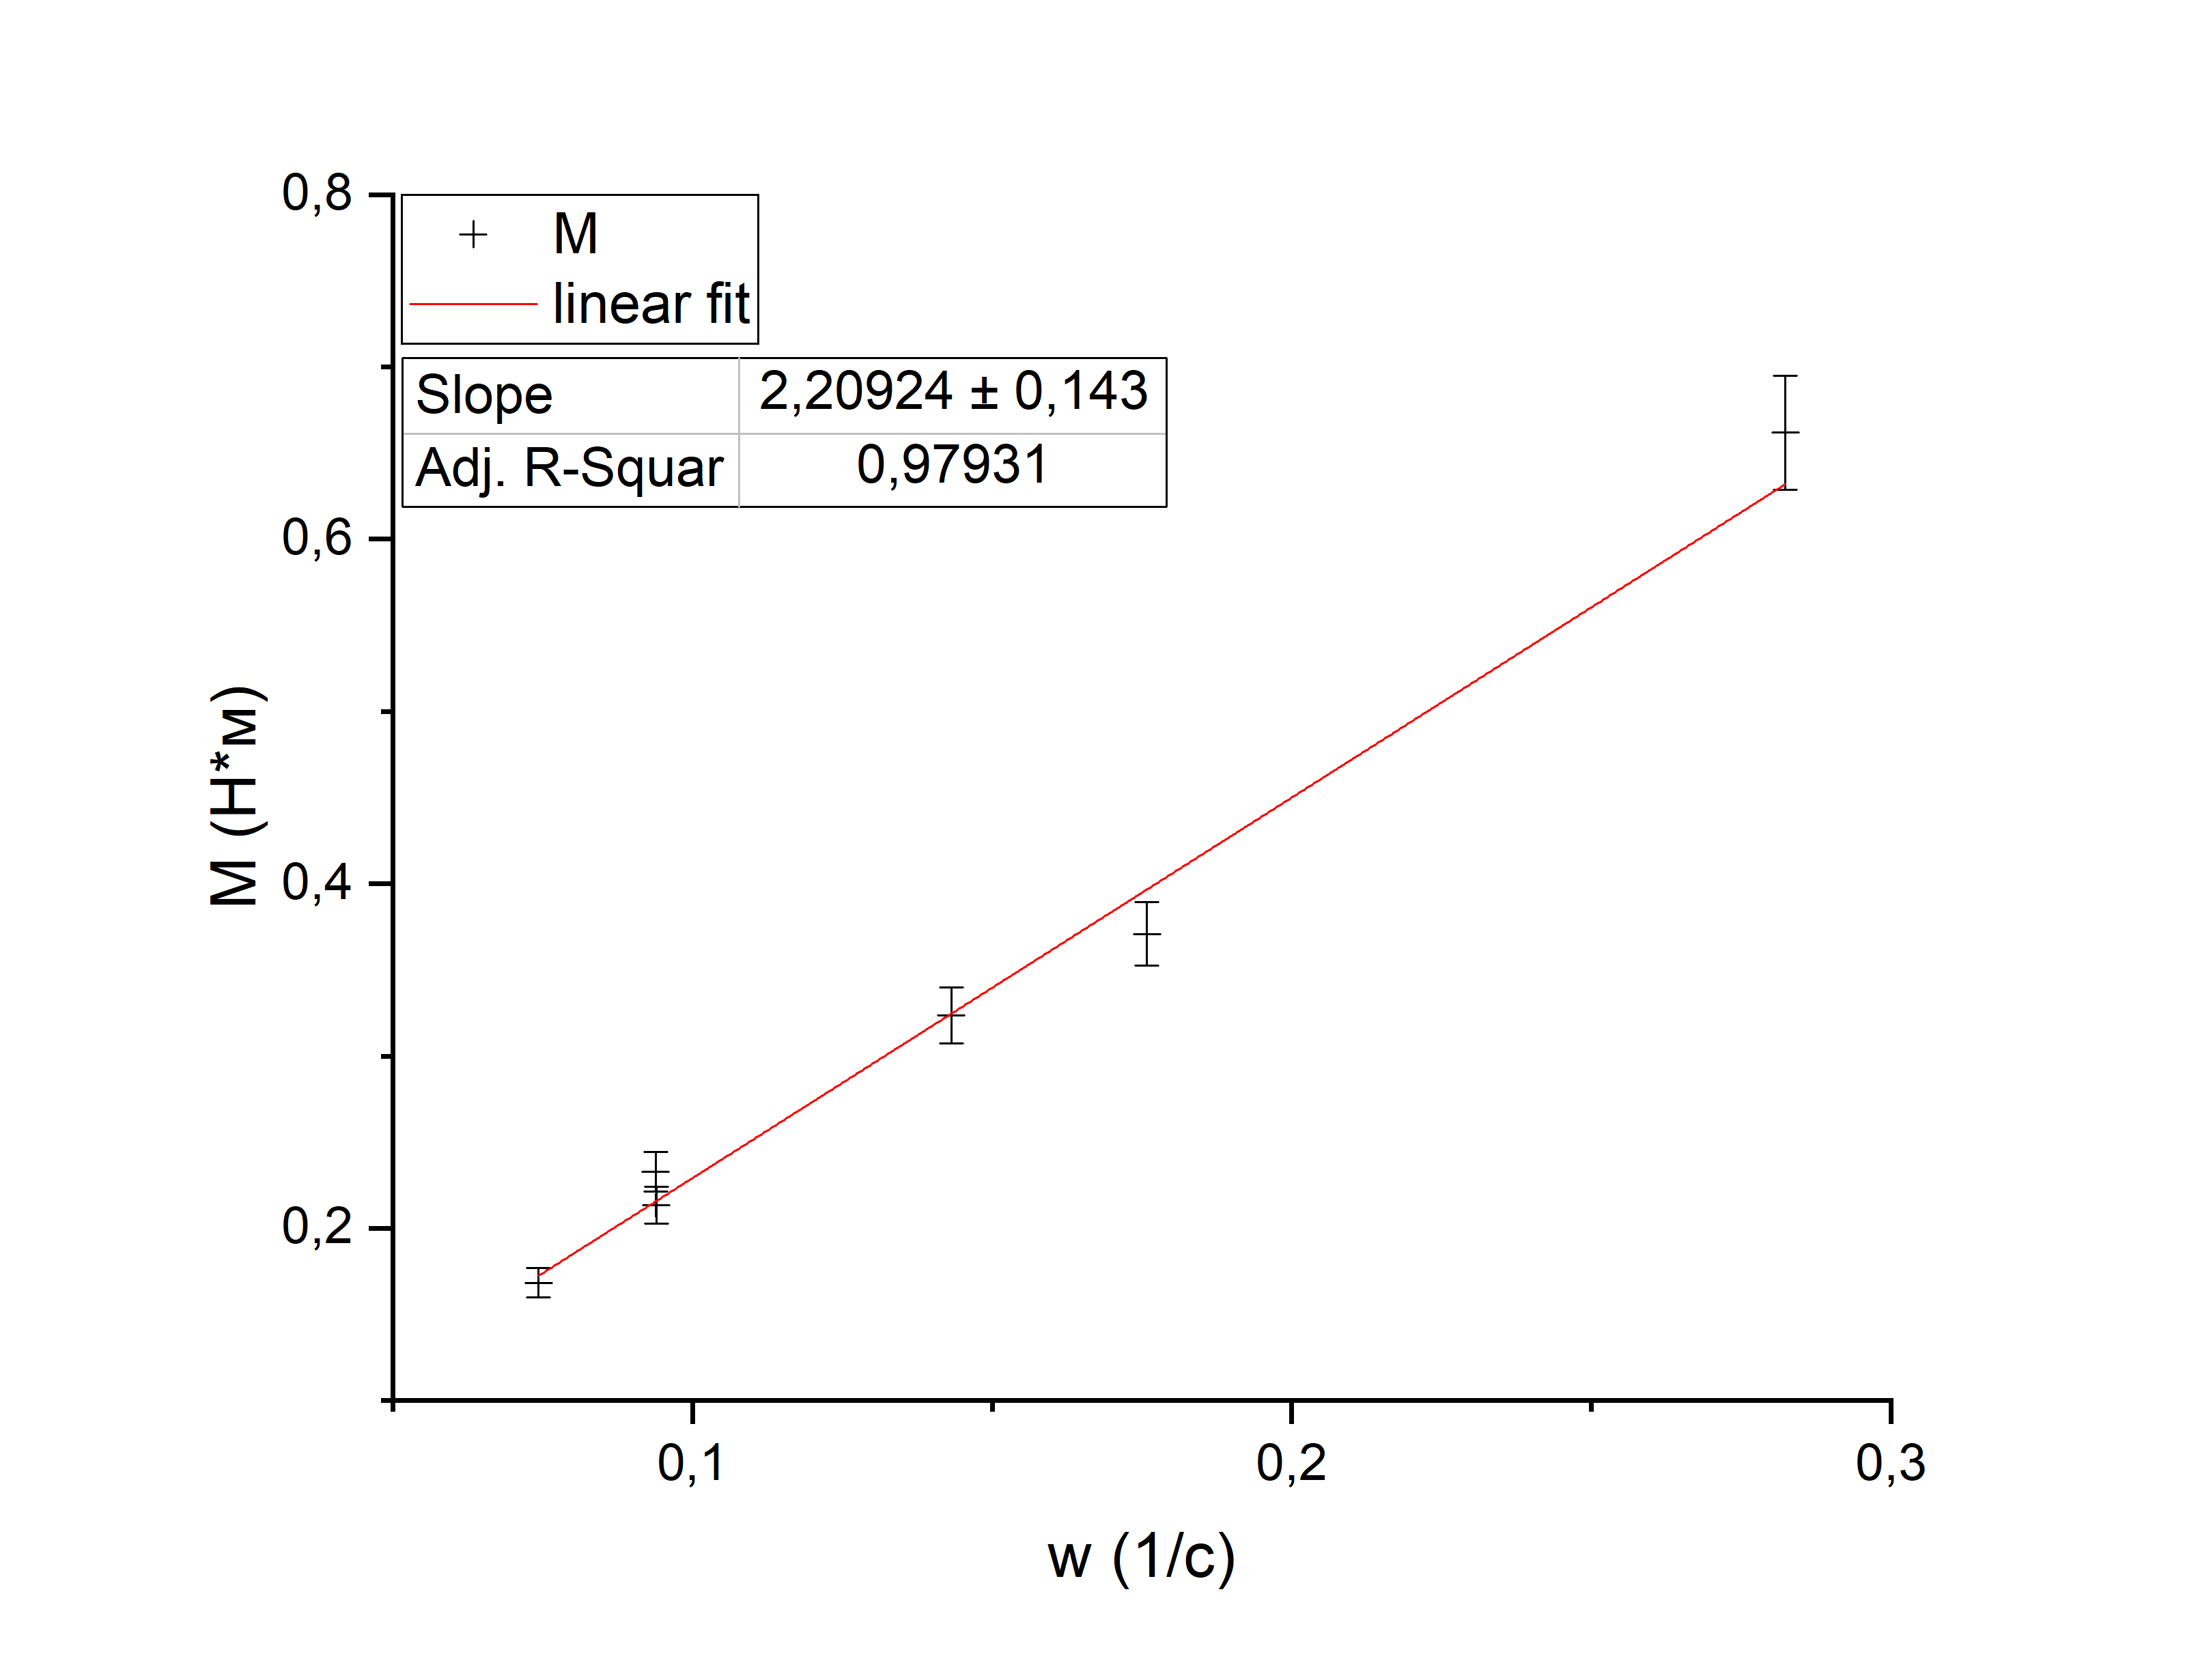
\includegraphics[width=\textwidth]{125_3.jpg}
\end{center}
\item Измеряем момент инерции $I_0$ относительно оси симметрии. Для этого подвешиваем ротор к концу вертикально висящей проволоки так, чтобы ось симметрии гироскопа была вертикальна, и измеряем период крутильных колебаний маятника $T_0$. Заменяем ротор на цилиндр известного радиуса и известной массы. 
\begin{center}

\begin{tabular}{|c|c|c|c||c|c|c|c|}
\hline
\multicolumn{4}{|c||}{Известный цилиндр}        & \multicolumn{4}{c|}{Ротор}             \\ \hline
           & $N$   & $t, c$   & $\sigma_t, c$  &         & $N$ & $t, c$ & $\sigma_t, c$ \\ \hline
1          & 10    & 32       & 0,1            & 1       & 10  & 42,2   & 0,1           \\ \hline
2          & 10    & 32,5     & 0,1            & 2       & 10  & 41,3   & 0,1           \\ \hline
3          & 10    & 32,7     & 0,1            & 3       & 10  & 41,3   & 0,1           \\ \hline
4          & 10    & 31,8     & 0,1            & 4       & 10  & 41,3   & 0,1           \\ \hline
5          & 10    & 32,2     & 0,1            & 5       & 10  & 41,3   & 0,1           \\ \hline
Среднее    & 10    & 32,24    & 0,15           & Среднее & 10  & 41,5   & 0,15          \\ \hline
\multicolumn{4}{|c||}{$T_c = (3,23 \pm 0,015) c$} & \multicolumn{4}{c|}{$T_0 = (4,146 \pm 0,016) c$} \\ \hline
\end{tabular}
\begin{tabular}{|c|c|c|c|c|c|}
\hline
\multicolumn{6}{|c|}{Параметры цилиндра}                                                          \\ \hline
$M, kg$ & $\sigma_M, kg$ & $R, kg$ & $\sigma_R, m$ & $I, kg \cdot m^2$ & $\sigma_I, kg \cdot m^2$ \\ \hline
1,618   & 0,001          & 0,0391  & 0,0001        & 0,00122            & 0,00007                   \\ \hline
\end{tabular}
\end{center}
Измеряем его период крутильных колебаний $T_c$ и по формуле 
\[I_0 = I_c \dfrac{T_0^2}{T_c^2}\] 
\[\sigma_{I_c} =I_c \sqrt{  \left( \dfrac{\sigma_M }{M} \right)^2 + 2  \left( \dfrac{ \sigma_R }{R} \right) ^2 } \]
\[\sigma_{I_0} = I_0 \sqrt{ 2 \left( \dfrac{\sigma_{T_c}}{T_c} \right) ^2 + 2 \left( \dfrac{\sigma_{T_0}}{T_0} \right) ^2 +  \left( \dfrac{\sigma_{I_c}}{I_c} \right) ^2}\]
измеряем $I_0 = (0,0012 \pm 0,0007) kg \cdot m^2$.
\item По формулам
\[\sigma_{\Omega} = \Omega \sqrt{\left( \dfrac{M/ \omega_0}{\sigma_{M/ \omega_0}} \right) ^2 + \left( \dfrac{I_0}{ \sigma_{I_0} } \right) ^2 }\]
\[\Omega = \dfrac{mgl}{I_0 w_0} = \dfrac{M}{I_0 \omega_0}\]
определяем частоту вращения гироскопа $\Omega = (3080 \pm 250) c^{-1}$.
\item По скорости опускания рычага определяем момент сил трения. 
\[M_{F_{frict}} = I_0 w_0 \Omega_{v} \]

\begin{center}
\begin{tabular}{|c|c|c|c|c|c|}
\hline
$\omega_0$ & $\sigma_{omega_0}, 10^{-5} \cdot c^{-1}$ & $\Omega_{down}, c^{-1}$ & $\sigma_{Omega_{down}}, c^{-1}$ & $M_{F_{frict}}, 10^{-7} \cdot H$ & $\sigma_{M_{F_{frict}}}, 10^{-8} \cdot H$ \\ \hline
0,09396    & 3,5                                      & 0,0049                  & 0,0004                          & 5,7                              & 6                                         \\ \hline
0,09383    & 4,7                                      & 0,0065                  & 0,0005                          & 7,6                              & 8                                         \\ \hline
0,2823     & 21                                       & 0,0098                  & 0,0008                          & 34,2                             & 34                                        \\ \hline
0,07434    & 3                                        & 0,0051                  & 0,0004                          & 4,7                              & 5                                         \\ \hline
0,1431     & 8                                        & 0,0074                  & 0,0006                          & 13,2                             & 13                                        \\ \hline
0,1758     & 10                                       & 0,0073                  & 0,0006                          & 15,9                             & 16                                        \\ \hline
\end{tabular}
\end{center}
\newpage
\item По фигурам Лиссажу на осцилографе определяем частоту вращения гироскопа. $\nu = 470 c^{-1}, \text{  } 2 \pi \nu = \Omega = 2951,6 c^{-1}$ \\
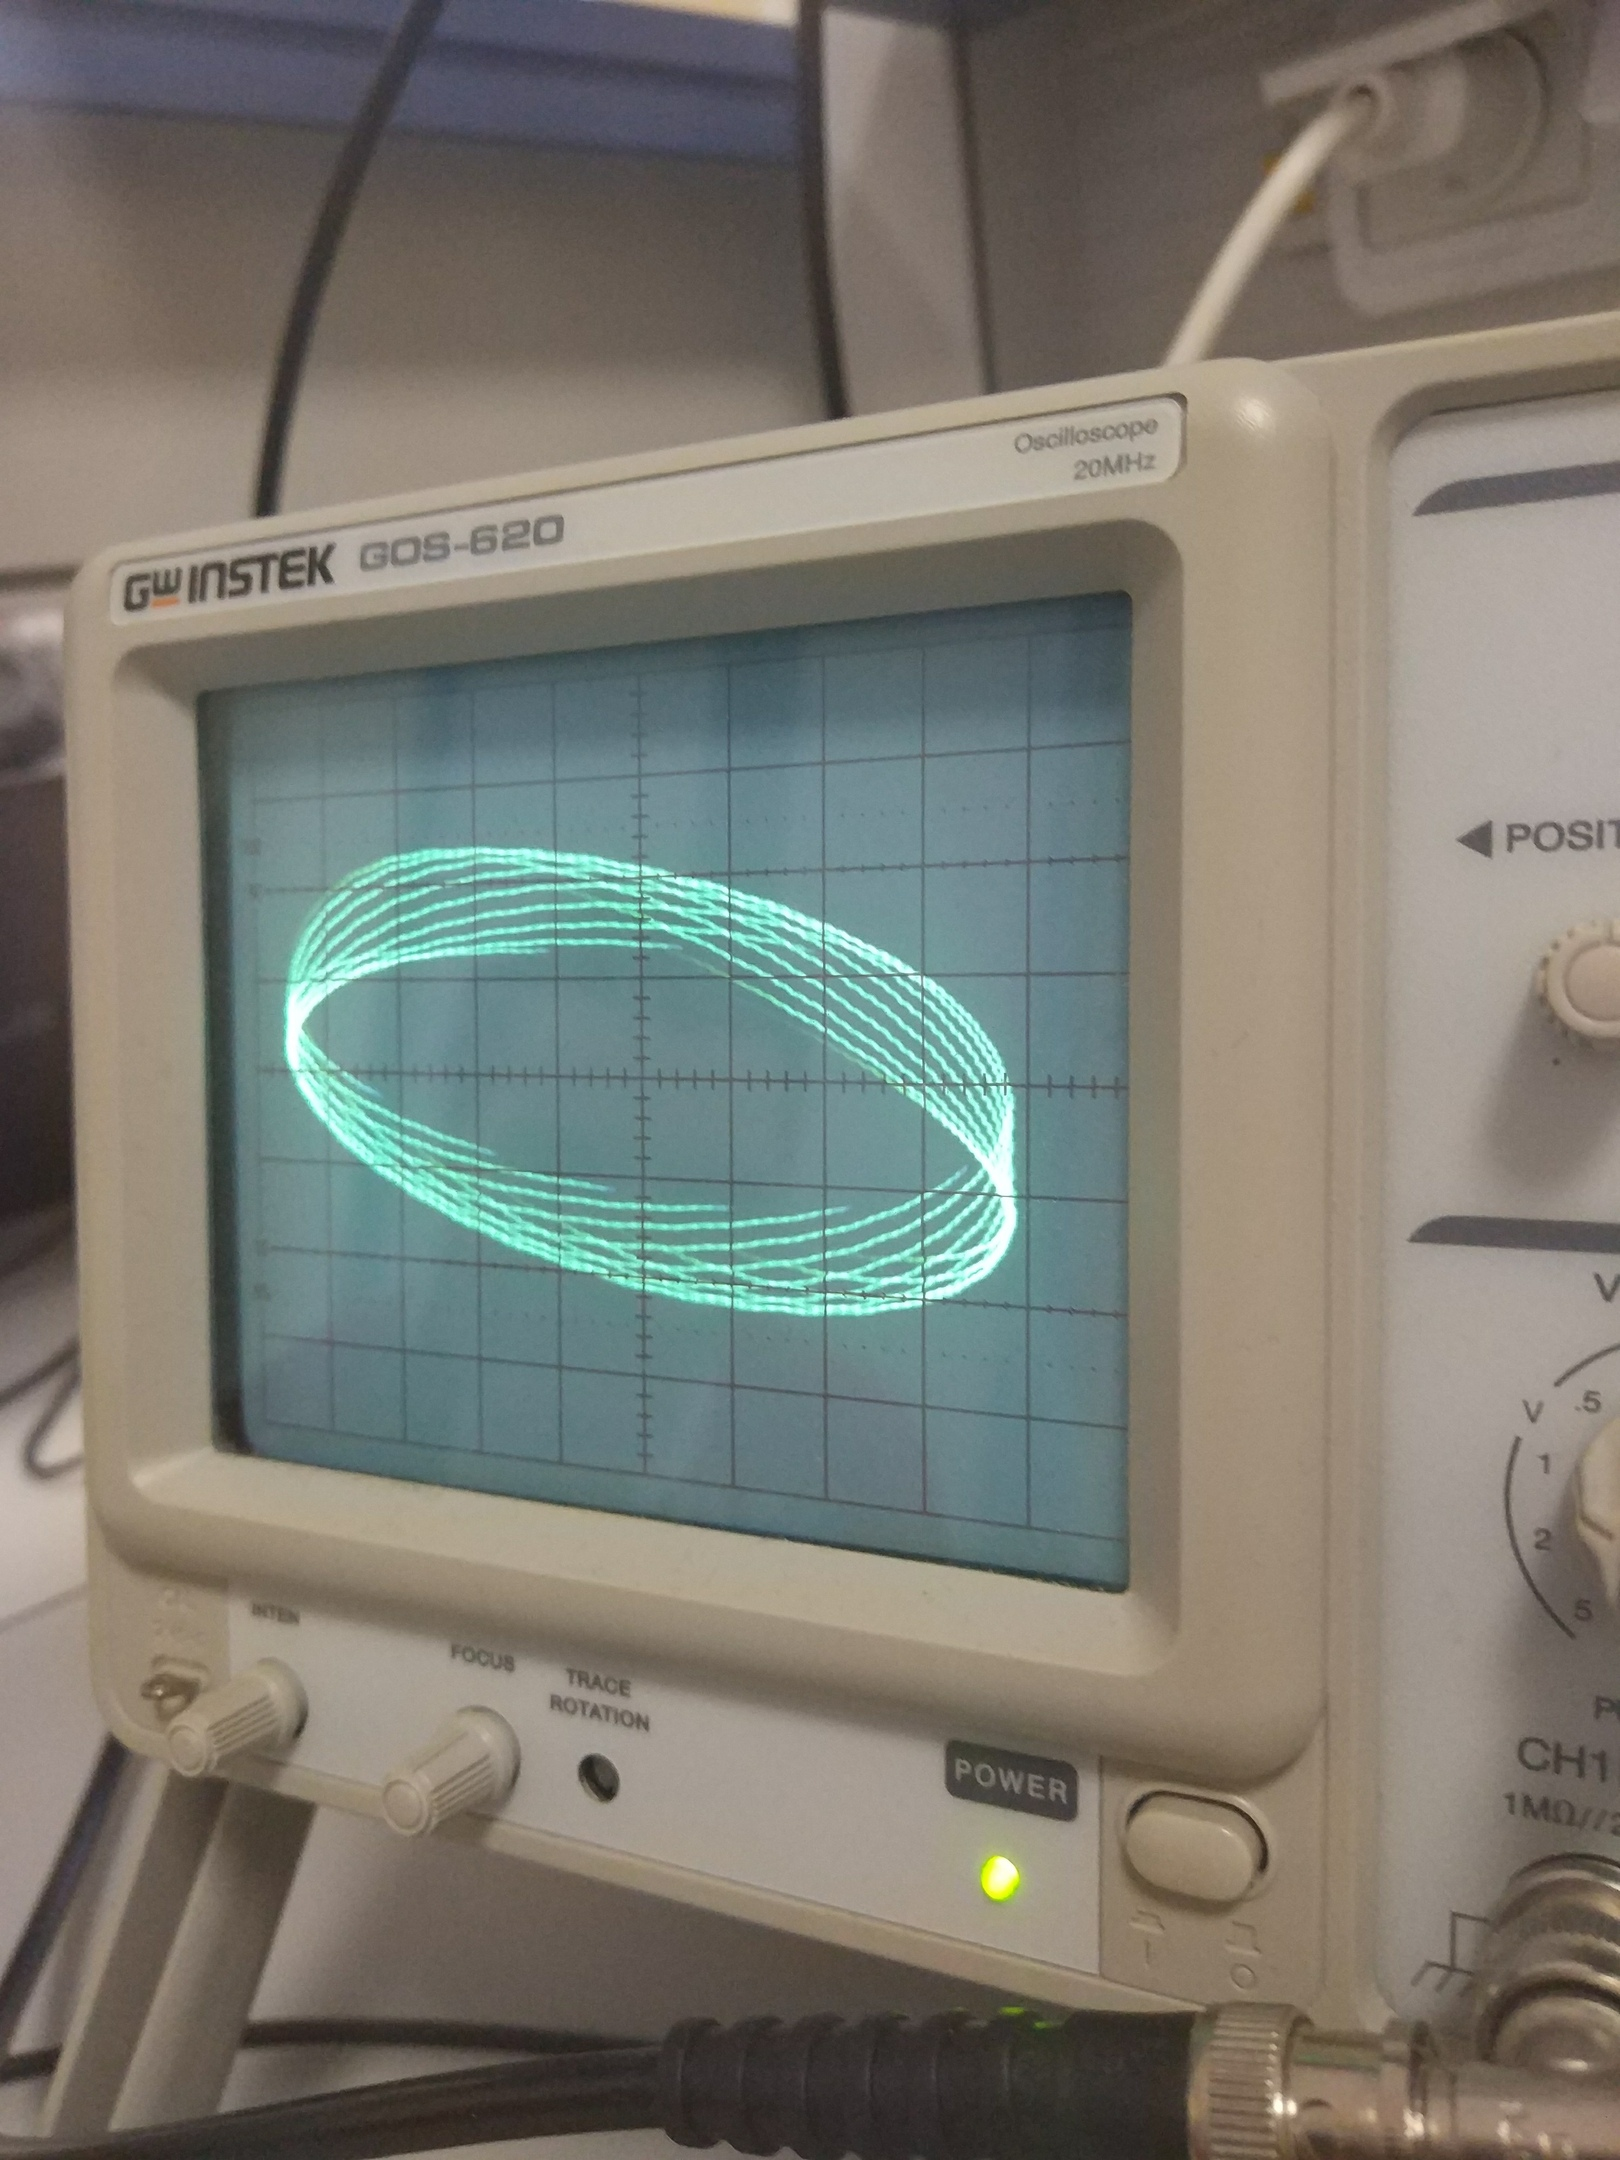
\includegraphics[width=0.4\textwidth]{125_4.jpg}
\item Убеждаемся, что $L_{\Omega} << L_{\sigma_0}$
\end{enumerate}
\end{document}